\documentclass[a4paper,12pt,french]{book}
\usepackage[margin=2cm]{geometry}
\usepackage[thinfonts]{uglix2}
\usepackage{ulem}
\nouveaustyle

\begin{document}
\titre{DS 03}{NSI}{2021}

\begin{center}
\textit{L'usage de la calculatrice n'est pas autorisé}\\[2em]
\end{center}

\section*{Exercice 1 \small{\hfill arbres binaires de recherche, langage objet}}
Dans cet exercice, les arbres binaires de recherche \textbf{ne peuvent pas comporter plusieurs fois la même clé}. De plus,\textbf{ un arbre binaire de recherche limité à un nœud a une hauteur de 1}.

On considère l’arbre binaire de recherche représenté ci-dessous, où \texttt{val} représente un entier :
\begin{center}
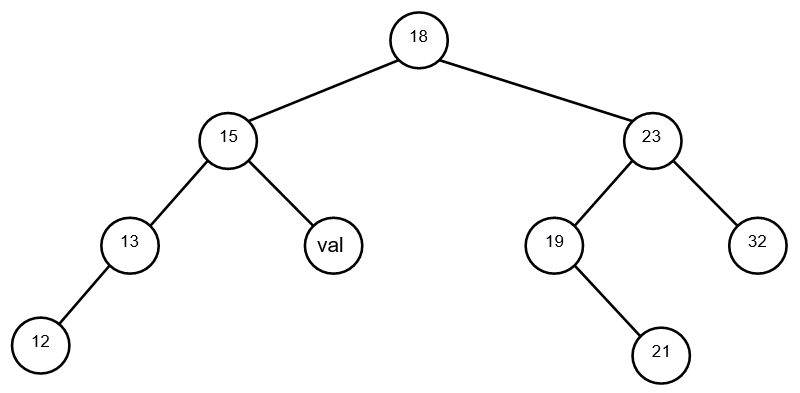
\includegraphics[width=10cm]{img/arbre}\\

Figure 1\\[1em]

\end{center}

\begin{enumerate}[\bfseries 1.]
	\item \begin{enumerate}[\bfseries a.]
    	\item Donner le nombre de feuilles de cet arbre et préciser leur valeur (étiquette).
        \item Représenter le sous arbre-gauche du nœud 23.
        \item Donner la hauteur et la taille de l’arbre.
        \item Donner les valeurs entières possibles de \texttt{val} pour cet arbre binaire de recherche.
    \end{enumerate}


    \item On suppose, pour la suite de cet exercice, que \texttt{val} est égal à 16.\\

        On rappelle qu’un parcours infixe depuis un nœud consiste, dans l’ordre, à faire un parcours infixe sur le sous arbre-gauche, afficher le nœud puis faire un parcours infixe sur le sous-arbre droit.
        Dans le cas d’un parcours suffixe (aussi appelé postfixe), on fait un parcours suffixe sur le sous-arbre gauche puis un parcours suffixe sur le sous-arbre droit, avant d’afficher le nœud.\\

            \begin{enumerate}[\bfseries a.]
            	\item Donner les valeurs d’affichage des nœuds dans le cas du parcours infixe de l’arbre.
                \item Donner les valeurs d’affichage des nœuds dans le cas du parcours suffixe de l’arbre.
            \end{enumerate}
\newpage
      \item On considère la classe \pythoninline{Noeud} définie ainsi :

\begin{pythoncode}
class Noeud():
    def __init__(self, v):
        self.ag = None
        self.ad = None
        self.v = v

    def insere(self, v):
        n = self
        est_insere = False
        while not est_insere :
            if v == n.v:
                est_insere = True       # Bloc 1 (une ligne)
            elif v < n.v:
                if n.ag != None:        # Bloc 2
                    n = n.ag            #
                else:                   #
                    n.ag = Noeud(v)     #
                    est_insere = True   # Fin bloc 2
            else:
                if n.ad != None:        # Bloc 3
                    n = n.ad            #
                else:                   #
                    n.ad = Noeud(v)     #
                    est_insere = True   # Fin bloc 3

    def insere_tout(self, vals):
        for v in vals:
            self.insere(v)
\end{pythoncode}

\begin{enumerate}[\bfseries a.]
	\item Représenter l'arbre construit suite à l'exécution des instructions suivantes :
    \begin{pythoncode}
racine = Noeud(18)
racine.insere_tout([12, 13, 15, 16, 19, 21, 32, 23])
    \end{pythoncode}
    \newpage
    \item \'Ecrire les deux instructions permettant de construire l’arbre de la figure 1. On rappelle que le nombre \texttt{val} est égal à 16.

    \item  On considère l’arbre tel qu’il est présenté sur la figure 1.\\
    Déterminer l’ordre d’exécution des blocs (repérés de 1 à 3) suite à l’application de la méthode \pythoninline{insere(19)} au nœud \pythoninline{racine} de cet arbre.
    \item \'Ecrire une méthode \pythoninline{recherche(self, v)} qui prend en argument un entier \pythoninline{v} et renvoie la valeur \pythoninline{True} si cet entier est une étiquette de l’arbre, \pythoninline{False} sinon.
\end{enumerate}
\end{enumerate}


\section*{Exercice 2 \small{\hfill gestion des processus}}

\subsection*{Partie A}

Cette partie est un questionnaire à choix multiples (QCM).\\
Pour chacune des questions, une seule des quatre réponses est exacte. Le candidat indiquera sur sa copie le numéro de la question et la lettre correspondant à la réponse exacte.
Aucune justification n’est demandée. Une réponse fausse ou une absence de réponse n’enlève aucun point.
\begin{enumerate}[\bfseries 1.]
	\item 	Parmi les commandes ci-dessous, laquelle permet d’afficher les processus en cours d’exécution ?
            \begin{multicols}{4}
             \textbf{a.} \texttt{dir}\\
                       \textbf{b.} \texttt{ps}\\
                        \textbf{c.} \texttt{man}\\
                        \textbf{d.} \texttt{ls}
            \end{multicols}


   \item Quelle abréviation désigne l’identifiant d’un processus dans un système d’exploitation de type UNIX ?
         \begin{multicols}{4}
                 \textbf{a.} \texttt{PIX}\\
                           \textbf{b.} \texttt{SIG}\\
                            \textbf{c.} \texttt{PID}\\
                            \textbf{d.} \texttt{SID}
                \end{multicols}


     \item Comment s’appelle la gestion du partage du processeur entre différents processus ?
         \begin{multicols}{4}
                 \textbf{a.} interblocage\\\
                           \textbf{b.} ordonnancement\\
                            \textbf{c.} planification\\
                            \textbf{d.} priorisation
                \end{multicols}

      \item Quelle commande permet de supprimer un processus dans un système d’exploitation de type UNIX ?

         \begin{multicols}{4}
                 \textbf{a.} \texttt{stop}\\
                           \textbf{b.} \texttt{interrupt}\\
                            \textbf{c.} \texttt{end}\\
                            \textbf{d.} \texttt{kill}
                \end{multicols}
\end{enumerate}
\subsection*{Partie B}
\begin{enumerate}[\bfseries 1.]
	\item 	 Un processeur choisit à chaque cycle d’exécution le processus qui doit être exécuté. Le tableau ci-dessous donne pour trois processus P1, P2, P3 :
        \begin{enumerate}[--]
        	\item 	la durée d’exécution (en nombre de cycles);
        	\item 	l’instant d’arrivée sur le processeur (exprimé en nombre de cycles à partir de 0);
            \item 	le numéro de priorité.
        \end{enumerate}
        Le numéro de priorité est d’autant plus petit que la priorité est grande.\\
        On suppose qu’à chaque instant, c’est le processus qui a le plus petit numéro de priorité qui est exécuté, ce qui peut provoquer la suspension d’un autre processus, lequel reprendra lorsqu'il sera le plus prioritaire.
        \begin{center}
        \begin{tabular}{|c|c|c|c|}
        \hline
        \rowcolor{UGLiOrange} \textbf{\color{white}Processus }& \textbf{\color{white}Durée d'exécution} & \textbf{\color{white}Instant d'arrivée} & \textbf{\color{white}Numéro de priorité} \\
        \hline
        P1 & 3 & 3 & 1 \\
        \hline
        P2 & 3 & 2 & 2  \\
        \hline
        P3 & 4 & 0 & 3  \\
        \hline
        \end{tabular}
        \end{center}
        Reproduire le tableau ci-dessous sur la copie et indiquer dans chacune des cases le processus exécuté à chaque cycle.
        \begin{center}
        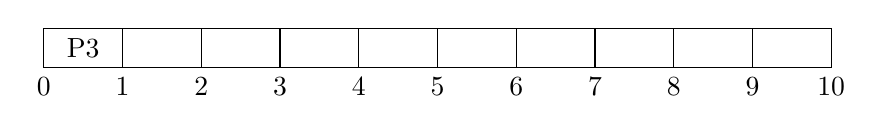
\begin{tikzpicture}
        \draw[xstep=1,ystep=.5] (0,0) grid (10,.5);
        \foreach \i in {0,1,...,10}
        {\draw(\i,0) node[below]{\i};}
        \draw (.5,.25) node {P3};
        \end{tikzpicture}
        \end{center}
	\item 	On suppose maintenant que les trois processus précédents s’exécutent et utilisent une ou plusieurs ressources parmi R1, R2 et R3.\\
    Parmi les scénarios suivants, lequel provoque un interblocage ? Justifier.
    \begin{center}
    	\begin{tabular}{|c|c|c|}
                \hline
                \rowcolor{UGLiOrange} \textbf{\color{white}Scénario 1 }& \textbf{\color{white}Scénario 2} & \textbf{\color{white}Scénario 3}  \\
                \hline
                P1 acquiert R1 & P1 acquiert R1 & P1 acquiert R1 \\
                \hline
                P2 acquiert R2& P2 acquiert R3 & P2 acquiert R2  \\
                \hline
                P3 attend R1& P3 acquiert R2 & P3 attend R2   \\
                \hline
                P2 libère R2& P1 attend R2 & P1 attend R2   \\
                                \hline
                P2 attend R1& P2 libère R3 & P2 libère R2   \\
                                \hline
                P1 libère R1& P3 attend  R1 & P3 acquiert R2   \\
                                \hline
                \end{tabular}
                \end{center}

\section*{Exercice 3 \small{\hfill binaire et logique}}
     Pour chiffrer un message, une méthode, dite du masque jetable, consiste à le combiner avec une chaîne de caractères de longueur comparable.
     Une implémentation possible utilise l’opérateur \texttt{XOR} (ou exclusif) dont voici la table de vérité :
    \begin{center}
    	\begin{tabular}{|c|c|c|}
                \hline
                \rowcolor{UGLiOrange} \textbf{\color{white}\texttt{a} }& \textbf{\color{white}\texttt{b}} & \textbf{\color{white}\texttt{a XOR b} }  \\
                \hline
                0 & 0 & 0 \\
                \hline
                0 & 1 & 1 \\
                \hline
                1 & 0 & 1 \\
                \hline
                1 & 1 & 0 \\
                \hline
                \end{tabular}
                \end{center}
   	Dans la suite, les nombres écrits en binaire seront précédés du préfixe \texttt{0b}.
       \begin{enumerate}[\bfseries 1.]
       	\item Pour chiffrer un message, on convertit chacun de ses caractères en binaire (à l’aide du format \textsc{Unicode}), et on réalise l’opération \texttt{XOR} bit à bit avec la clé.\\

                Après conversion en binaire, et avant que l’opération XOR bit à bit avec la clé n’ait été effectuée, Alice obtient le message suivant :

           \begin{center}
           \texttt{m = 0b 0110 0011 0100 0110}
           \end{center}
           \begin{enumerate}[\bfseries a.]
           	\item 	Le message \texttt{m} correspond à deux caractères codés chacun sur 8 bits : déterminer quels sont ces caractères. On fournit pour cela la table ci-dessous qui associe à l’écriture hexadécimale d’un octet le caractère correspondant. \\[.5em]
            \begin{center}
            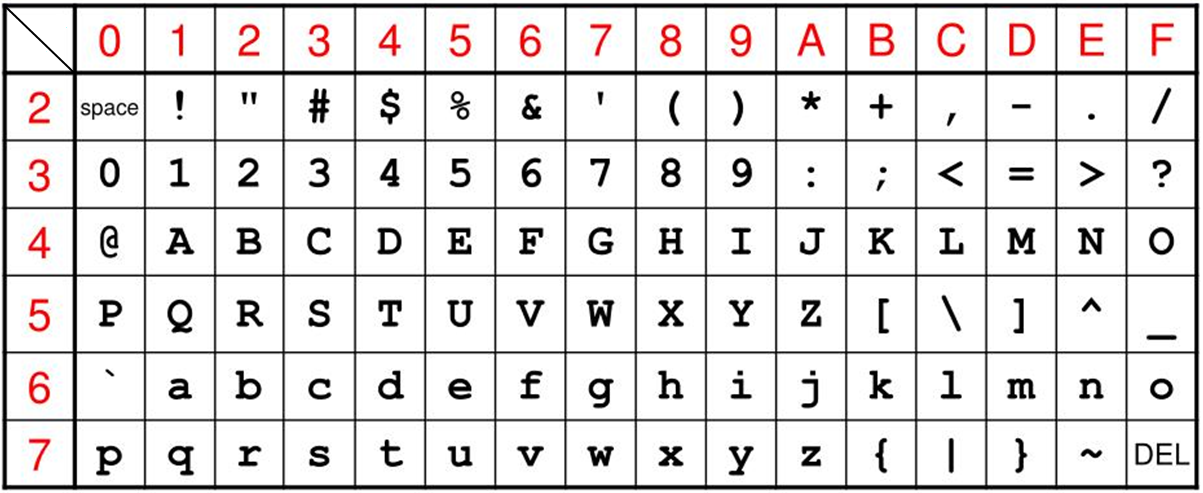
\includegraphics[width=10cm]{img/ascii}\\
            \end{center}
            \textit{\footnotesize Exemple de lecture : le caractère correspondant à l’octet codé \texttt{4A} en hexadécimal est la lettre \texttt{J}.}\\
           	\item Pour chiffrer le message d’Alice, on réalise l’opération \texttt{XOR} bit à bit avec la clé suivante :
               \begin{center}
               \texttt{k = 0b 1110 1110 1111 0000}
               \end{center}
               Donner l’écriture binaire du message obtenu.
           \end{enumerate}

       	\item 	\begin{enumerate}[\bfseries a.]
           	\item 	Donner la table de vérité de l'expression booléenne \texttt{(a XOR b) XOR b}.
           	\item 	Bob connaît la chaîne de caractères utilisée par Alice pour chiffrer le message. Quelle opération doit-il réaliser pour déchiffrer son message ?

           \end{enumerate}
       \end{enumerate}
\end{enumerate}




\end{document}